\documentclass{article}
 % Some basic packagesLLuu
\usepackage[utf8]{inputenc}
\usepackage[margin=1.2in]{geometry}
\usepackage{textcomp}
\usepackage{url}
\usepackage{graphicx}
\usepackage{float}
\usepackage{enumitem}
\usepackage{standalone}
\usepackage{tcolorbox}
\usepackage{wrapfig}
\usepackage{pgfplots} 
% \pgfplotset{compat=1.8}
% \pgfplotsset{scaled y ticks=false}
% \usepackage{svg}
% \usepackage{svg-inkscape} 

%color settings
\usepackage{xcolor}
\definecolor{gruvbgdark}{HTML}{1d2021}
\definecolor{gruvtextdark}{HTML}{ebdbb2}
\definecolor{gruvbglight}{HTML}{f9f5d7}
\definecolor{gruvtextlight}{HTML}{3c3836}
\definecolor{NavyBlue}{HTML}{266bbd}
\definecolor{RawSienna}{HTML}{94330e}
\definecolor{ForestGreen}{HTML}{149b52}
% \pagecolor{gruvbgdark}
% \color{gruvtextdark}

% Hide page number when page is empty
\usepackage{emptypage}
\usepackage{subcaption}
\usepackage{multicol}

% Math stuff
\usepackage{amsmath, amsfonts, mathtools, amsthm, amssymb}
% Fancy script capitals
\usepackage{mathrsfs}
\usepackage{cancel}

% Bold math
\usepackage{bm}

% SVG setup
% \svgsetup{inkscapeexe=inkscape, inkscapearea=drawing}
% \svgpath{~/dev/DAVE3700-Matte-3000/figures/}

% Some shortcuts
\newcommand\N{\ensuremath{\mathbb{N}}}
\newcommand\R{\ensuremath{\mathbb{R}}}
\newcommand\Z{\ensuremath{\mathbb{Z}}}
\renewcommand\O{\ensuremath{\emptyset}}
\newcommand\Q{\ensuremath{\mathbb{Q}}}
\newcommand\C{\ensuremath{\mathbb{C}}}

%Make implies and impliedby shorter
\let\implies\Rightarrow
\let\impliedby\Leftarrow
\let\iff\Leftrightarrow

\let\epsilon\varepsilon

% Add \contra symbol to denote contradiction
% \usepackage{stmaryrd} % for \lightning
% \newcommand\contra{\scalebox{1.5}{$\lightning$}}

\let\phi\varphi

% Command for short corrections
% Usage: 1+1=\correct{3}{2}

\definecolor{correct}{HTML}{009900}
\newcommand\correct[2]{\ensuremath{\:}{\color{red}{#1}}\ensuremath{\to }{\color{correct}{#2}}\ensuremath{\:}}
\newcommand\green[1]{{\color{correct}{#1}}}

% horizontal rule
% \newcommand\hr{
%     \noindent\rule[0.5ex]{\linewidth}{0.5pt}
% }

% hide parts
\newcommand\hide[1]{}

% Environments
\makeatother

% For box around Definition, Theorem, \ldots
% theorems
\usepackage{thmtools}
\usepackage[framemethod=TikZ]{mdframed}
\mdfsetup{skipabove=1em,skipbelow=1em, innertopmargin=5pt, innerbottommargin=6pt}

\theoremstyle{definition}

\makeatletter

% \declaretheoremstyle[headfont=\bfseries, bodyfont=\normalfont, mdframed={ nobreak } ]{thmgreenbox}
% \declaretheoremstyle[headfont=\bfseries, bodyfont=\normalfont, mdframed={ nobreak } ]{thmredbox}
% \declaretheoremstyle[headfont=\bfseries, bodyfont=\normalfont, spaceabove=0.5cm, spacebelow=0.5cm]{thmbluebox}
% % \declaretheoremstyle[headfont=\bfseries, bodyfont=\normalfont]{thmbluebox}
% \declaretheoremstyle[headfont=\bfseries, bodyfont=\normalfont]{thmblueline}
% \declaretheoremstyle[headfont=\bfseries, bodyfont=\normalfont, numbered=no, mdframed={ rightline=false, topline=false, bottomline=false, }, qed=\qedsymbol ]{thmproofbox}
% \declaretheoremstyle[headfont=\bfseries\sffamily, bodyfont=\normalfont, numbered=no, mdframed={ nobreak, rightline=false, topline=false, bottomline=false } ]{thmexplanationbox}
\declaretheoremstyle[headfont=\bfseries, bodyfont=\normalfont, numbered=no]{idea}

\declaretheoremstyle[
	headfont=\bfseries\color{ForestGreen!70!black}, bodyfont=\normalfont,
	mdframed={
			linewidth=2pt,
			rightline=false, topline=false, bottomline=false,
			linecolor=ForestGreen, backgroundcolor=ForestGreen!5,
		}
]{thmgreenbox}

\declaretheoremstyle[
	headfont=\bfseries\color{NavyBlue!70!black}, bodyfont=\normalfont,
	mdframed={
			linewidth=2pt,
			rightline=false, topline=false, bottomline=false,
			linecolor=NavyBlue, backgroundcolor=NavyBlue!5,
		}
]{thmbluebox}

\declaretheoremstyle[
	headfont=\bfseries\color{NavyBlue!70!black}, bodyfont=\normalfont,
	mdframed={
			linewidth=2pt,
			rightline=false, topline=false, bottomline=false,
			linecolor=NavyBlue
		}
]{thmblueline}

\declaretheoremstyle[
	headfont=\bfseries\color{RawSienna!70!black}, bodyfont=\normalfont,
	mdframed={
			linewidth=2pt,
			rightline=false, topline=false, bottomline=false,
			linecolor=RawSienna, backgroundcolor=RawSienna!5,
		}
]{thmredbox}

\declaretheoremstyle[
	headfont=\bfseries\color{RawSienna!70!black}, bodyfont=\normalfont,
	numbered=no,
	mdframed={
			linewidth=2pt,
			rightline=false, topline=false, bottomline=false,
			linecolor=RawSienna, backgroundcolor=RawSienna!0,
		},
	qed=\qedsymbol
]{thmproofbox}

\declaretheoremstyle[
	headfont=\bfseries\color{NavyBlue!70!black}, bodyfont=\normalfont,
	numbered=no,
	mdframed={
			linewidth=2pt,
			rightline=false, topline=false, bottomline=false,
			linecolor=NavyBlue, backgroundcolor=NavyBlue!1,
		},
]{thmexplanationbox}

\declaretheorem[style=thmgreenbox, name=Definisjon]{definition}
\declaretheorem[sibling=definition, style=thmredbox, name=Corollary]{corollary}
\declaretheorem[style=idea, name=Idea]{idea}
\declaretheorem[style=idea, style=thmredbox, name=Proposition]{prop}
\declaretheorem[sibling=definition, style=thmredbox, name=Theorem]{theorem}
\declaretheorem[sibling=definition, style=thmredbox, name=Lemma]{lemma}



\declaretheorem[numbered=no, style=thmexplanationbox, name=Proof]{explanation}
\declaretheorem[numbered=no, style=thmproofbox, name=Proof]{replacementproof}
\declaretheorem[style=thmbluebox,  numbered=no, name=Exercise]{ex}
\declaretheorem[style=thmbluebox,  numbered=no, name=Svar]{ans}
\declaretheorem[style=thmbluebox,  numbered=no, name=Example]{eg}
\declaretheorem[style=thmblueline, numbered=no, name=Remark]{remark}
\declaretheorem[style=thmblueline, numbered=no, name=Note]{note}

\renewenvironment{proof}[1][\proofname]{\begin{replacementproof}}{\end{replacementproof}}

\AtEndEnvironment{eg}{\null\hfill$\diamond$}%

\newtheorem*{uovt}{UOVT}
\newtheorem*{notation}{Notation}
\newtheorem*{previouslyseen}{As previously seen}
\newtheorem*{problem}{Problem}
\newtheorem*{observe}{Observe}
\newtheorem*{property}{Property}
\newtheorem*{intuition}{Intuition}


% Exercise 
% Usage:
% \oefening{5}
% \suboefening{1}
% \suboefening{2}
% \suboefening{3}
% gives
% Oefening 5
%   Oefening 5.1
%   Oefening 5.2
%   Oefening 5.3
\newcommand{\oefening}[1]{%
	\def\@oefening{#1}%
	\subsection*{Oefening #1}
}

\newcommand{\suboefening}[1]{%
	\subsubsection*{Oefening \@oefening.#1}
}


% \lecture starts a new lecture (les in dutch)
%
% Usage:
% \lecture{1}{di 12 feb 2019 16:00}{Inleiding}
%
% This adds a section heading with the number / title of the lecture and a
% margin paragraph with the date.

% I use \dateparts here to hide the year (2019). This way, I can easily parse
% the date of each lecture unambiguously while still having a human-friendly
% short format printed to the pdf.

% \usepackage{xifthen}
% \def\testdateparts#1{\dateparts#1\relax}
% \def\dateparts#1 #2 #3 #4 #5\relax{
% 	\marginpar{\small\textsf{\mbox{#1 #2 #3 #5}}}
% }

% \def\@lecture{}%
% \newcommand{\lecture}[3]{
% 	\ifthenelse{\isempty{#3}}{%
% 		\def\@lecture{Lecture #1}%
% 	}{%
% 		\def\@lecture{Lecture #1: #3}%
% 	}%
% 	\subsection*{\@lecture}
% 	% \marginpar{\small\textsf{\mbox{#2}}}
% }

\usepackage{listings}
\usepackage{color}

\definecolor{dkgreen}{rgb}{0,0.6,0}
\definecolor{gray}{rgb}{0.5,0.5,0.5}
\definecolor{mauve}{rgb}{0.58,0,0.82}

\lstset{frame=tb,
  language=Java,
  aboveskip=3mm,
  belowskip=3mm,
  showstringspaces=false,
  columns=flexible,
  basicstyle={\small\ttfamily},
  numbers=none,
  numberstyle=\tiny\color{gray},
  keywordstyle=\color{blue},
  commentstyle=\color{dkgreen},
  stringstyle=\color{mauve},
  breaklines=true,
  breakatwhitespace=true,
  tabsize=3
}


% These are the fancy headers
\usepackage{fancyhdr}
\pagestyle{fancy}

% LE: left even
% RO: right odd
% CE, CO: center even, center odd
% My name for when I print my lecture notes to use for an open book exam.
\fancyhead[LE,RO]{Kristian Sørdal}

\fancyhead[RO,LE]{INF102 - Algoritmer og Data Strukturer} % Right odd,  Left even
\fancyhead[RE,LO]{\leftmark}          % Right even, Left odd

\fancyfoot[RO,LE]{\thepage}  % Right odd,  Left even
\fancyfoot[RE,LO]{}          % Right even, Left odd
\fancyfoot[C]{\leftmark}     % Center

\makeatother

% Todonotes and inline notes in fancy boxes
\usepackage{todonotes}
\usepackage{tcolorbox}

% Make boxes breakable
\tcbuselibrary{breakable}

% Figure support as explained in my blog post.
\usepackage{import}
\usepackage{xifthen}
\usepackage{pdfpages}
\usepackage{transparent}
\newcommand{\incfig}[2][1]{%
	% \begin{center}
	\def\svgwidth{#1\columnwidth}
	\import{./figures/}{#2.pdf_tex}
	% \end{center}
}

\graphicspath{{./figures/}}
% Fix some stuff
% %http://tex.stackexchange.com/questions/76273/multiple-pdfs-with-page-group-included-in-a-single-page-warning
\pdfsuppresswarningpagegroup=1
\author{Kristian Sørdal}


\begin{document}
\section{Eksamen Høst 2020}
    \subsection{Oppgave 1}
    Hva er kjøretiden til denne koden?

    \begin{lstlisting}
public double interestOnLoan(double amount, int n) {
    amount = amount * 1.01; 
}
return amount
    \end{lstlisting}

    \begin{ans}
        \[ O(n) \]
    \end{ans}

    \subsection{Oppgave 2}
    Hva er kjøretiden til denne koden?

    \begin{lstlisting}
public static int countOneBits(int n) {
    int bits = 0;
    while (n > 0) {
        if (n % 2 == 1) {
            bits++;
        }
        n = n / 2;
    }
    return bits;
}
    \end{lstlisting}

    \begin{ans}
        \[ O\left( \log n  \right) \]
    \end{ans}

    \subsection{Oppgave 3}
    Hva er kjøretiden til denne koden?
        
    \begin{lstlisting}
public static int countSteps (int n) {
    int pow = 2;
    int steps = 0;

    for(int i = 0; i < n; i++) { // n
        if (i == pow) { // n
            pow *= 2;
            for(int j = 0; j < n; j++) {
                steps++;
            }
        } else {
            steps++;
        }
    }
    return steps;
} 
    \end{lstlisting}

    \begin{ans}
        \[ O\left( n \log n \right) \]
    \end{ans}

    \subsection{Oppgave 4}
    Hva er kjøretiden til denne koden?
    \begin{lstlisting}
public staic String makeRandomString(int n) {
    String ans = "";
    for (int i = 0; i < n; i++) {
        char c = (char) ('a'+26*Math.random());
        ans += c;
    }
    return ans;
    
} 
    \end{lstlisting}

    \begin{ans}
        \[ O(n^2) \]
    \end{ans}

    \subsection{Oppgave 5}
    Hva er kjøretiden til denne koden?

    \begin{lstlisting}
public static double computeAreaUnderCurve(LinkedList<Double> y) {
    Double area = 0.0;

    for(int i = 1; i < y.size(); i++) {
        area = area + (y.get(i - 1) + y.get(i)) / 2;
    }
    return area;
}
    \end{lstlisting}

    \begin{ans}
        \[ O(n^2) \]
    \end{ans}

    \subsection{Oppgave 6}
    Hva er kjøretiden til denne koden?
    \begin{lstlisting}
// n = list.size() 
public static Collection<Integer> findLargestK(ArrayList<Integer> list, int k) {
    PriorityQueue<Integer> pq = new PriorityQueue<Integer>();
    for(int num: list) { // n
        if(pq.size() < k || pq.peek() < num) { // 1
            pq.add(num) // log k
        }

        if(pq.size() > k) { // 1
            pq.poll(); // log k
        }
    }
    return pq;
}
    \end{lstlisting}
    Har kan du anta at \( k < n \).

    \begin{ans}
        \[ O\left( n \log\left( k \right) \right) \]
    \end{ans}

    \subsection{Oppgave 7}
    Denne koden kalles når \texttt{words} er tom og vil da fylle inn settet \texttt{words}. Hva er kjøretiden til denne koden?

    \begin{lstlisting}
HashSet<String> dictionary;        
HashSet<String> words;

// n = dictionary.size()
// k = letters.length()

private void possibleWords(String word, String letters) {
    if(!word.isBlank() && dictionary.contains(word)) { // n
        words.add(word); // 1
    }

    int k = letters.length(); // 1

    for(int i = 0; i < k; i ++) { // k
        // add letter to word
        String nextWord = word + letters.charAt(i); // k

        // remove letter from available letters
        String nextLetters = letters.substring(0, i); 

        if (i < k - 1) {
            nextLetters = nextLetters + letters.substring(i + 1, k);
        }

        // continue searching
        possibleWords(nextWord, nextLetters);
    }
}
    \end{lstlisting}

    Her kan du anta at \( k < n \).

    \begin{ans}
        \[ O\left( k! \cdot  k  \right) \]
        
    \end{ans}

    \subsection{Oppgave 8}
    Forklar hvordan algoritmen \texttt{QuickSort} ville sortert denne listen med tall.

    \[ 4,7,15,1,9,3,6,12,2 \]

    \begin{ans}

        \texttt{QuickSort} bruker en \texttt{pivot} for å dele opp listen i verdier som er større enn og mindre enn denne verdien. Sorteringen vil skje på følgende måte: Som første pivot vil vi bruke veriden lengst til høyre i listen. Høyre og venstre er de indeksene i listen som vi foreløpig ser på, og er initalisert til 0 og lengden av listen - 1, som i dette tilfellet er 8.

        \begin{table}[H]
            \begin{center}
                \begin{tabular}[c]{|l|l|l|l|}
                    \hline
                    Liste&Pivot&Høyre&Venstre  \\
                    \hline
                     4,7,15,1,9,3,6,12,2&2&0&9  \\
                    \hline
                     1,2,4,3,6,7,9,12,15&7&2&8 \\
                    \hline
                     1,2,4,3,6,7,9,12,15&6&2&4 \\
                    \hline
                     1,2,3,4,6,7,9,12,15&3&2&3 \\
                    \hline
                     1,2,3,4,6,7,9,12,15&15&6&8 \\
                    \hline
                     1,2,3,4,6,7,9,12,15&12&6&7 \\
                    \hline
                \end{tabular}
            \end{center}
        \end{table}
        
    \end{ans}

    \subsection{Oppgave 9}
    DFS (dybde først søk) er en metode for å besøke alle nodene i en graf. Hver node blir kun besøkt en gang. Forklar hvordan DFS kjører på denne grafen ved å stegvis beskrive hva algoritmen gjør og i hvilken rekkefølge nodene vil bli besøkt. Du skal begynne søket i node "a". Det er mange rette rekkefølger, du skal bare gi en mulig rekkefølge for DFS.

    \begin{figure}[H]
        \begin{center}
            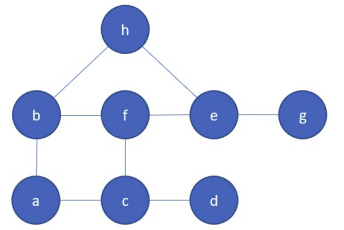
\includegraphics[width=0.45\textwidth]{dfsgraph9}
        \end{center}
    \end{figure}

    \begin{ans}
        DFS opererer på \textit{Last in, First out} prinsippet. Den vil derfor besøke alle nodene i siten til et løv, før den går videre opp i grafen og finner andre noder. Vi kan beskrive rekkefølgen og hva algoritmen gjør i en tabell.

        \begin{table}[H]
            \begin{center}
                \begin{tabular}[c]{|l|l|l|l|}
                    \hline
                    Nåværende node& Neste node & Kø & Besøkte  \\
                    \hline
                      a&b&c,b& \\
                    \hline
                      b&h&c,f,h&a \\
                    \hline
                      h&e&c,f,e&a,b \\
                    \hline
                      e&g&c,f,f,g&a,b,h \\
                    \hline
                      g&f&c,f,f&a,b,h,e \\
                    \hline
                      f&c&c,f,c&a,b,h,e,g \\
                    \hline
                      c&d&c,f,d&a,b,h,e,g,f \\
                    \hline
                      d&&c,f&a,b,h,e,g,f,c \\
                    \hline
                      &&&a,b,h,e,g,f,c,d \\
                    \hline
                \end{tabular}
            \end{center}
        \end{table}
    \end{ans}

\subsection{Oppgave 10}
BFS (bredde først søk) er en metode for å besøke alle nodene i en graf. Hver node blir kun besøkt en gang. Forklar hvordan BFS kjører på denne rettede grafen ved å beskrive hvilken rekkefølge nodene vil bli besøkt. Du skal begynne søket i node "a". Det er mange rette svar du skal bare gi en mulig rekkefølge for BFS.



\begin{figure}[H]
    \begin{center}
        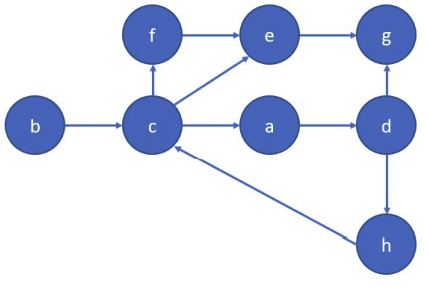
\includegraphics[width=0.45\textwidth]{bfsgraph10}
    \end{center}
\end{figure}

\begin{ans}
    BFS opererer på \textit{First in, First out} prinsippet, og vi kan beskrive hva algoritmen gjør med en tabell
        \begin{table}[H]
            \begin{center}
                \begin{tabular}[c]{|l|l|l|l|}
                    \hline
                    Nåværende node& Neste node & Kø & Besøkte  \\
                    \hline
                      a&d&d&\\
                    \hline
                      d&g&g,h&a\\
                    \hline
                      g&h&h,c&a,d\\
                    \hline
                      h&c&c&a,d,g\\
                    \hline
                      c&f&f,a&a,d,g,h\\
                    \hline
                      f&e&a,e&a,d,g,h,c\\
                    \hline
                      e&&a&a,d,g,h,c,f\\
                    \hline
                      &&&a,d,g,h,c,f,e\\
                    \hline
                \end{tabular}
            \end{center}
        \end{table}
\end{ans}
\end{document}
